\chapter{Technische Umsetzung} \label{implementation}

Die Implementation hat zum Ziel, die bereits erarbeitete konzeptionelle Lösung in Form von Code praktisch umzusetzen. Nach einer Übersicht über die abgeschlossene Visualisierung und einem Einblick in die eingesetzten Technologien wird im Detail auf nennenswerte Eigenheiten des Projektes eingegangen.

% -------------------------------

\section{Übersicht}


    \begin{figure}[H]
    \centering
    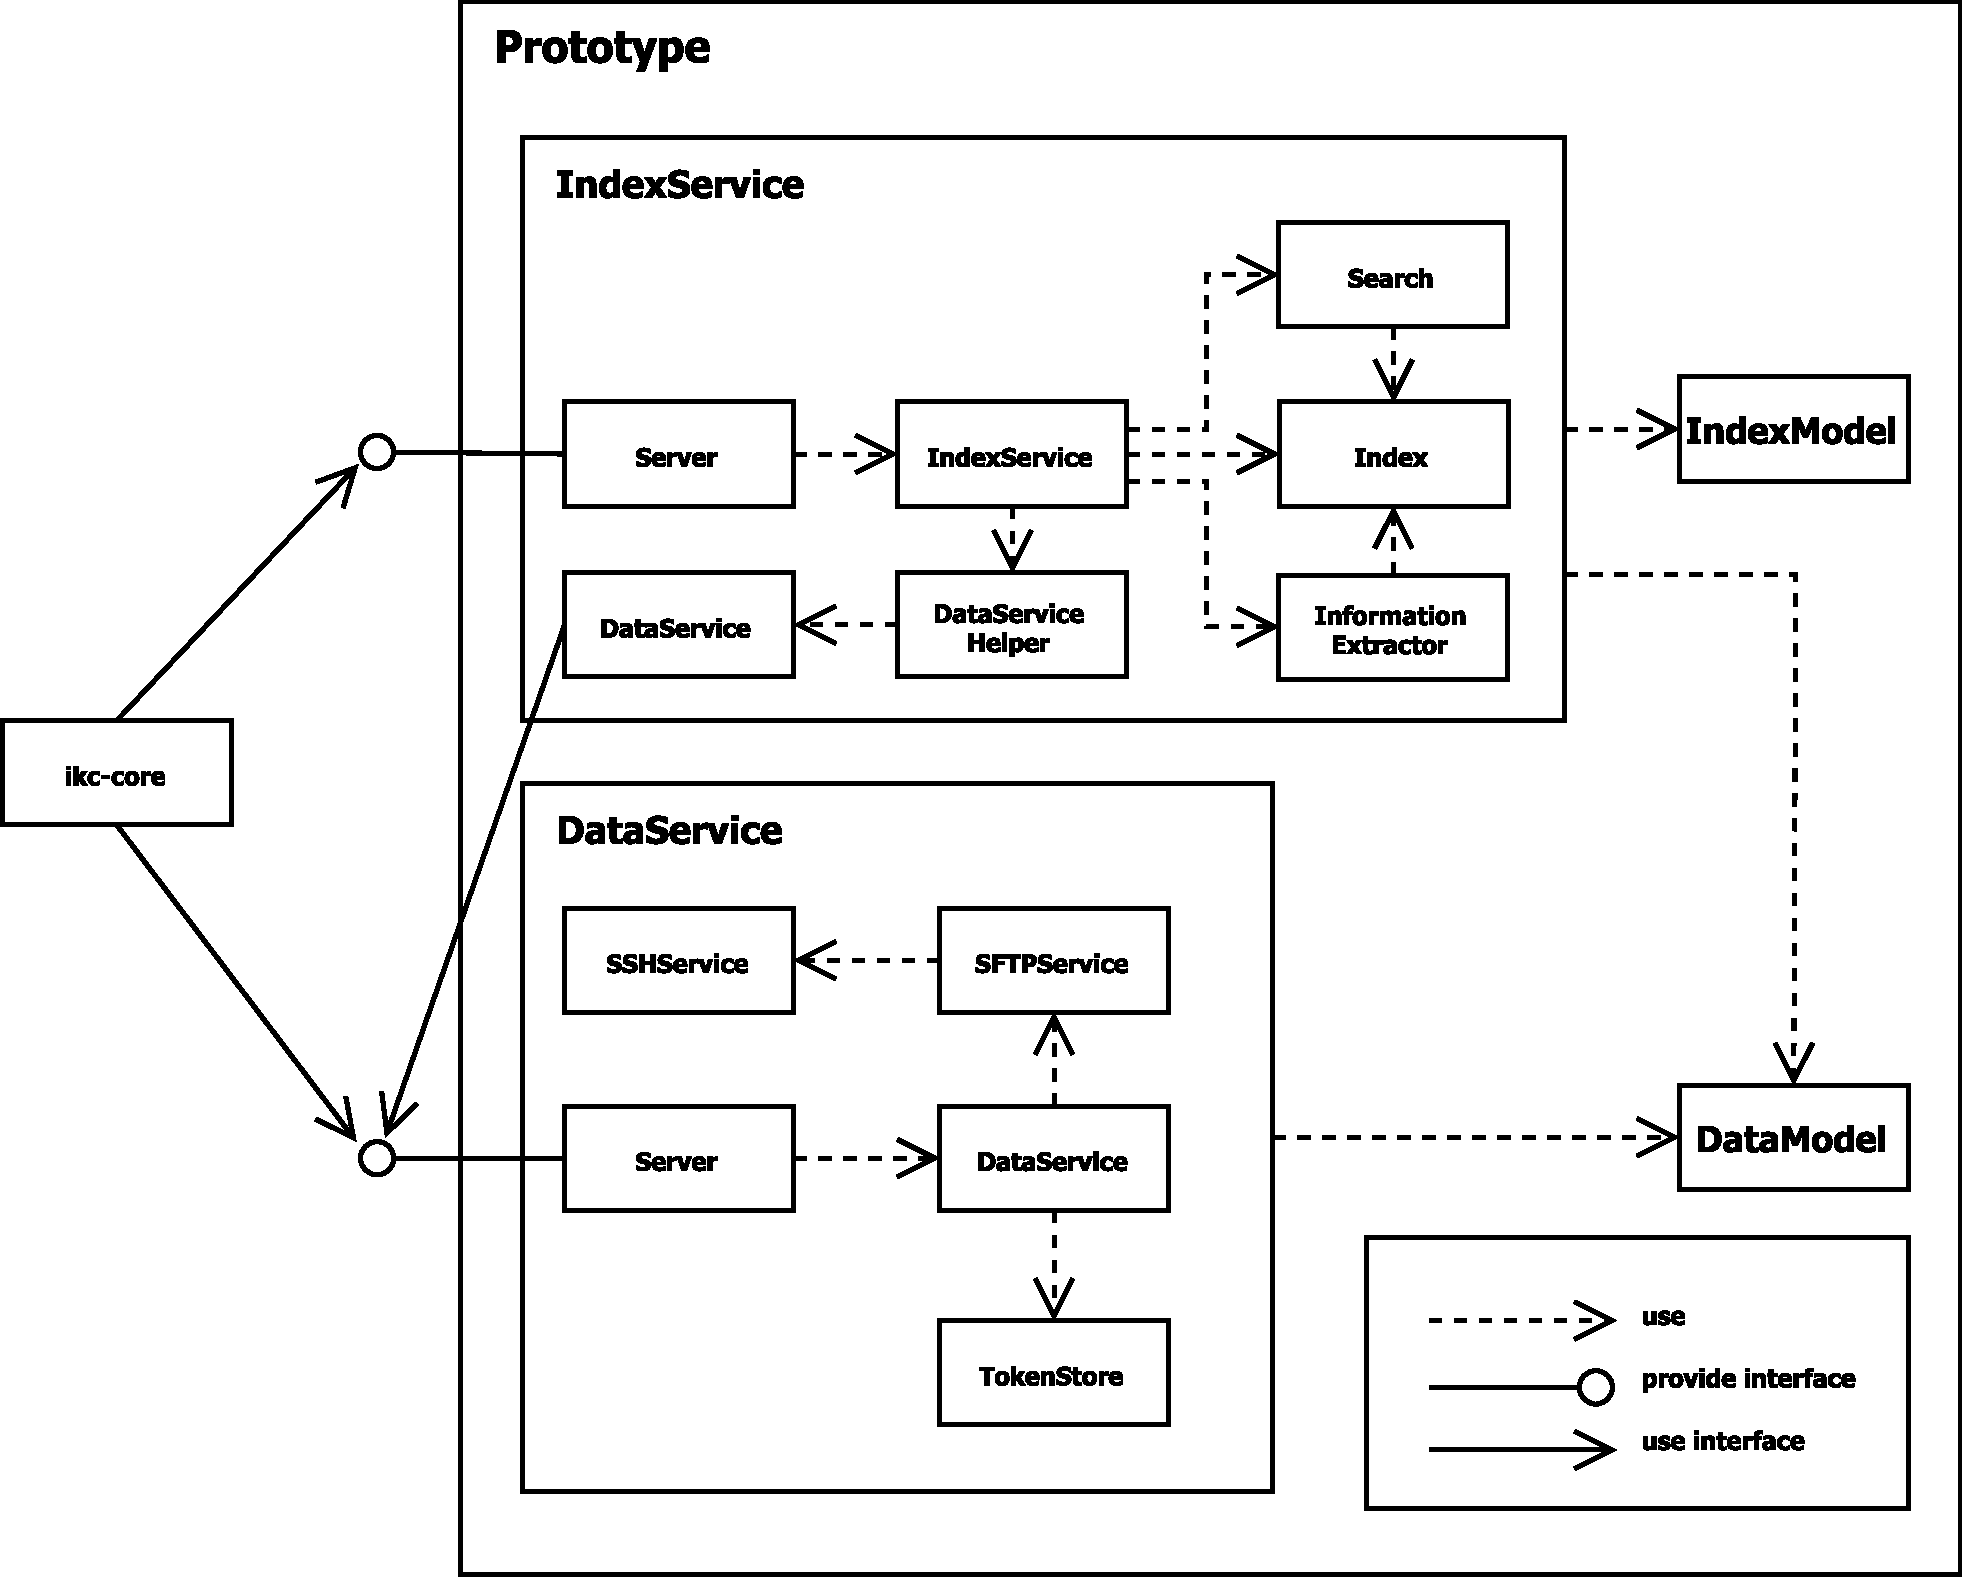
\includegraphics[width=1\textwidth]{PrototypeClassDiagram}
    \caption{Prototype Klassendiagram}
    \label{fig:prototypeClassDiagram}
    \end{figure}

Der Kern der Software bildet der Algorithmus, dieser ist, neben der Suchfunktionalität und dem Aufbau der Indizes, ein Hauptbestandteil des \texttt{IndexService}. \autoref{fig:kommunikation} gewährt einen Überblick über die beteiligten Komponenten. Als Grundlage benötigt der \texttt{In\-dex\-Ser\-vice} alle zu indexierenden Dateien im Volltext. Deren Quelle ist der \texttt{Data\-Ser\-vice}. Der \texttt{Index-} und der \texttt{DataService} bilden zusammen den eigentlichen Prototypen. Wie in der Bausteinsicht auf \autoref{fig:bausteinsicht} zu erkennen, gibt es neben der Integration der Services auch eine Einbindung in die bestehende Benutzeroberfläche des \gls{ikc-core}.

Folgend eine kurze Erklärung zu den einzelnen Klassen des \texttt{Index-} beziehungsweise \texttt{DataServices}.


\subsection{IndexService}

\texttt{IndexService}:
\begin{itemize}
    \item \textbf{Server}: Hier werden Netzwerk-Anfragen vom \gls{ikc-core} entgegengenommen. Und gegebenenfalls wird eine Antwort zu\-rück\-ge\-schi\-ckt.
    \item \textbf{IndexService}: Dies ist der Kern des \texttt{IndexService}: Anfragen können direkt an die Klasse \texttt{Index} weitergeleitet werden, falls der \texttt{Index} bereits geladen und verfügbar ist. Ist dies nicht der Fall oder soll eine Datei oder ein Verzeichnis gelesen werden, wird die Anfrage an den \texttt{DataServiceHelper} weitergeleitet.
    \item \textbf{DataServiceHelper}: Anfragen an den \texttt{DataService} müssen zu\-nä\-chst aufbereitet und wie nötig verpackt werden, das geschieht hier.
    \item \textbf{DataService}: Ist die Anfrage bereit verschickt zu werden, üb\-er\-ni\-mmt dies der \texttt{DataService}. Er übermittelt die Anfragen über das Netzwerk und nimmt die Antworten entgegen.
    \item \textbf{Search}: Der \texttt{IndexService} kann Suchanfragen mittels dem Voll\-te\-xt-Index verarbeiten und beantworten. Für diese Funktionalität steht die Klasse \texttt{Search} zur Verfügung.
    \item \textbf{Index}: Die Klasse \texttt{Index} hält die verschiedenen Index. Sie ist eine reine Datenklasse, bietet somit keine weitere Funktionalität, sondern repräsentiert den geladenen Index innerhalb der Applikation.
    \item \textbf{InformationExtractor}: Hier läuft der gesamte Prozess der Key\-wo\-rd-\-Ex\-trac\-ti\-on ab: Mit Hilfe des \texttt{Index} werden hier Schlüs\-sel\-wör\-ter extrahiert oder zu Schlü\-ssel\-wör\-tern passende Dokumente gefunden.
\end{itemize}

\subsection{DataService}

\texttt{DataService}:
\begin{itemize}
    \item \textbf{Server}: Auch hier hat der \texttt{Server} wiederum die Aufgabe Anfragen entgegenzunehmen und zu beantworten.
    \item \textbf{DataService}: Der \texttt{DataService} ist die Hauptklasse. Hier ist die zentrale Applikationslogik enthalten, Anfragen werden weitergeleitet. Die Anbindungen an eine Datenquelle wird ebenfalls von hier aus gesteuert.
    \item \textbf{TokenStore}: Das Zugriffskonzept mittels \gls{Token}[s] benötigt eine Zwischenspeicherung der Freigabeberechtigungen. Dies findet hier statt. 
    \item \textbf{SFTPService}: Ein Beispiel für eine externe Datenquelle ist \gls{SFTP}. Da der Zugriff hierbei über \gls{SSH} zu erfolgen hat, fungiert diese Klasse hier als Adapter.
    \item \textbf{SSHService}: Hier findet der eigentliche Zugriff auf die externe Datenquelle statt. Die Kommunikation geschieht über einen \gls{SSH}-Tunnel.
\end{itemize}

\subsection{Integration des Prototypen}
Der Prototyp soll sich möglichst Nahtlos in den \gls{ikc-core} integrieren. Um dies zu erreichen sollen in keiner Situation Funktionen des \gls{ikc-core} blockiert werden durch den Prototypen. 

So werden Suchresultate des Index innerhalb der bestehenden Suche integriert und bei Bedarf aktualisiert. Die verschieden Resultate der verschiedenen Quellen sollen in Echtzeit nach ihrem Eintreffen dargestellt werden. Somit wird sich die Liste mit Resultate trotz gleichem Suchbegriff über die Zeit verändern, da weitere Resultate von entfernten Quellen eintreffen. 

Weiter sollen extrahierte \gls{Keyword}[s] klar getrennt von den bestehenden Properties des Nodes als \textit{Chips} oberhalb des Titel dargestellt werden. Sowohl ein Dokument mit entsprechenden \gls{Keyword}[s] als auch eine \gls{Keyword} mit den verknüpften Dokumenten werden als Node dargestellt. \autoref{fig:bda_ui} zeigt einen Entwurf dieser Integration. 

    \begin{figure}[H]
    \centering
    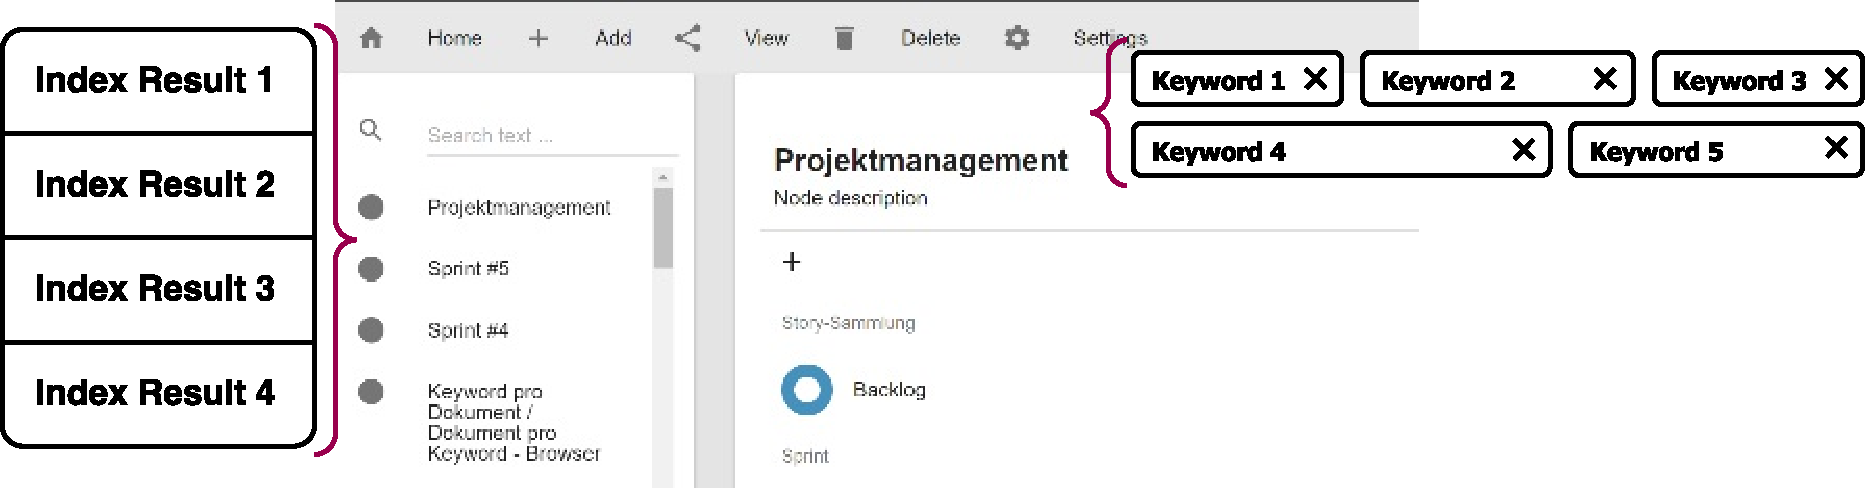
\includegraphics[width=1\textwidth]{BDA_UI}
    \caption{Entwurf Intgeration Benutzeroberfläche}
    \label{fig:bda_ui}
    \end{figure}

Um die Schnittstellen des Prototype ideal zu verwenden und die obigen Oberflächenanpassungen umzusetzten, sind Anpassungen bzw. Erweiterungen in der Software Struktur des \gls{ikc-core} nötig. Das Klassendiagramm (\autoref{fig:classDiagrammIkcCore}) erläutert die wichstigsten Anpassungen:

\begin{itemize}
    \item Um lokale Suchresultate mit denen des Volltext Indexes zu kombinieren wird die \texttt{SearchBroker} Klasse verwendet. Darin werden Resultate beider Quellen entgegengenommen und für die Darstellung verarbeitet. Mit Hilfe des Interface \texttt{SearchResult} und den beiden Implementierungen \texttt{IndexSearchResult} und \texttt{LocalSearchResult} sollen für den unterschiedlichen Umgang unterschiedenen werden. Sobald die ersten Suchresultate eintreffen werden diese verarbeitet und der Benutzeroberfläche weitergegeben. Durch die Generalisierung mittels dem Interface ist es weiter möglich beliebigen Suchquellen in unbegrenzter Anzahl zu integrieren. Er wird direkt von den Benutzeroberflächen Komponenten verwendet. 
    \item Der \texttt{IndexSearchService} ist verantwortlich für die Kommunikation mit dem \texttt{IndexService} als auch dem \texttt{DataService}. Dazu werden die vorgestellten Protokolle (\autoref{section:protokoll}) verwendetet.
    \item Um  dem Benutzer entfernte Nodes zu präsentieren wird der \texttt{ElementCache} verwendet. Darin werden temporäre Nodes des Index (Dokument oder \gls{Keyword}) gespeichert und bei Bedarf für die Benutzeroberfläche bereit gestellt.
    \item Der \texttt{IndexResultProcessor} bildet das Bindeglied zwischen Resultaten des \texttt{IndexService} und dem \texttt{ElementCache}. Er nimmt Resultate des \texttt{IndexService} von dem \texttt{IndexSearchService} entgegen, verarbeitet sie und sendet sie weiter an den \texttt{ElementCache}, wo sie anschliessend der Benutzeroberfläche zu Verfügung stehen.

\end{itemize}


    \begin{figure}[H]
    \centering
    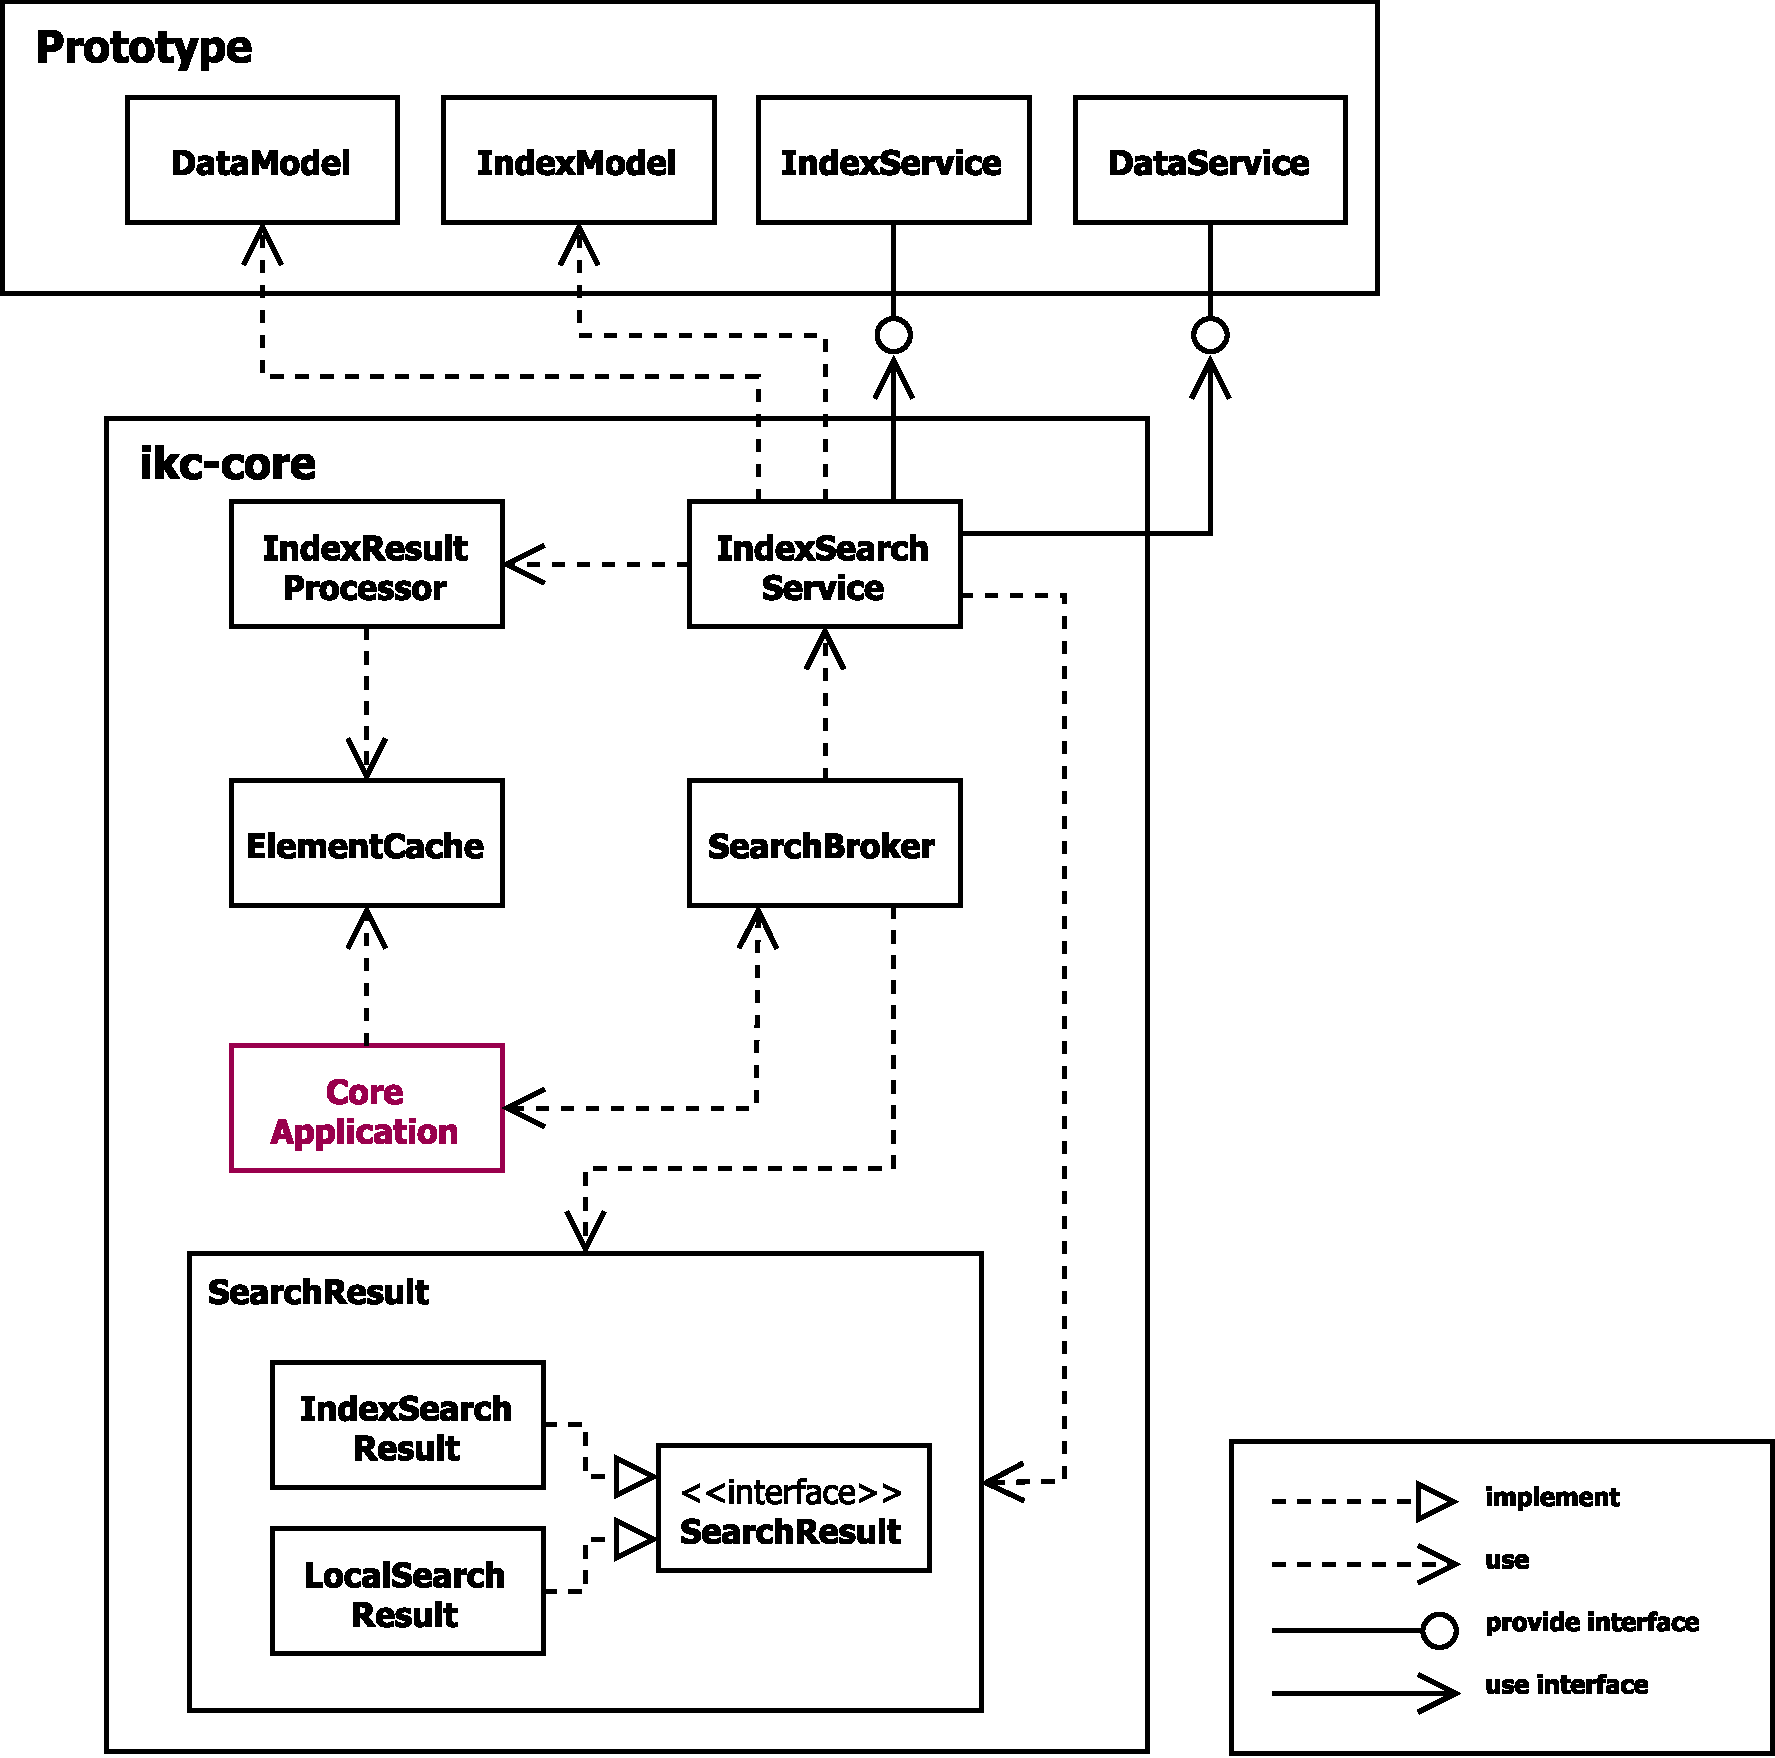
\includegraphics[width=1\textwidth]{ClassDiagrammIkcCore}
    \caption{Klassendiagramm Integration}
    \label{fig:classDiagrammIkcCore}
    \end{figure}
%riesiges index.json, ungefähr 100k Files als Text-Dateien

\subsection{Datenfreigabe}
Für den Auftraggeber ist eine sichere Kommunikation und stetige Transparenz und Kontrolle über den Verbleib von benutzergenerierten Daten von hoher Wichtigkeit. Um diesen Anforderungen gerecht zu werden, wurde unter anderem ein Datenfreigabe-Konzept entwickelt. Dieses basiert auf \gls{Token}[s]. Die Vorgehensweise kann mittels der \autoref{fig:seqaccesssession} gut aufgezeigt werden.

\begin{itemize}
    \item \texttt{requestToken}: Ein generischer Kunde (\texttt{<<customer>>}) möchte eine Datei von der externen Datenquelle beziehen. Zunächst muss er dafür den \texttt{Da\-ta\-Ser\-vi\-ce} für einen Freigabe-\gls{Token} anfragen. Dabei müssen bei der Anfrage Informationen, wie die gesamte Zugriffsberechtigung (\textit{Host}, \textit{User}, \textit{SSH-PrivateKey}) und der Pfad der Datei mitgegeben werden. Die Zugriffsberechtigung muss eigenhändig vom Benutzer hinterlegt werden.
    
    \item \texttt{generateToken}: Der \texttt{DatService} verarbeitet die Anfrage und generiert mit den gegebenen Informationen ein \gls{Token}.
    
    \item \texttt{storeToken}: Dieser \gls{Token} wird im Hintergrund mit der zu\-ge\-höri\-gen Zugangsberechtigung und dem Dateipfad für spätere Verwendung im \texttt{TokenStore} hinterlegt.
    
    \item \texttt{token}: Nun wird der \gls{Token} als Antwort auf die Anfrage an den generischen Kunden zurückgeschickt.
    
    \item \texttt{dataRequest}: Prinzipiell kann nun jeder generische Kunde mit dem erhaltenen \gls{Token} eine Dateianfrage an den \texttt{DataService} tätigen. Dies kann er tun, ohne Kenntnis über die Zugangsberechtigung zu haben. Der \gls{Token} ist ausreichend. Aber Achtung: Die vergebenen \gls{Token}[s] sind nur für einen Zugriff gültig (one-way). Nach dem ersten Gebrauch werden diese, und auch die zugehörigen Zugriffsberechtigungen, verworfen!
    \texttt{getPathForToken}: Der \texttt{DataService} sucht im \texttt{TokenStore} die zum \gls{Token} zu\-ge\-hör\-igen Daten. Dazu zählen einerseits die Zugangsberechtigung zur Datenquelle und andererseits der Dateipfad.
    
    \item \texttt{path}: Diese Daten werden an den \texttt{DataService} retourniert.
    \item \texttt{read}: Nun kann der \texttt{DataService} die Daten von der externen Datenquelle anfordern.
    \item \texttt{data}: Auf die Anfrage folgt eine Antwort, welche die ge\-wünsch\-ten Daten zurückliefert.
    \item \texttt{dataResponse}: Diese werden an den Kunden zurückgegeben.

\end{itemize}


%ablaufdiagramm Einwegtoken Entkopplung

    \begin{figure}[H]
    \centering
    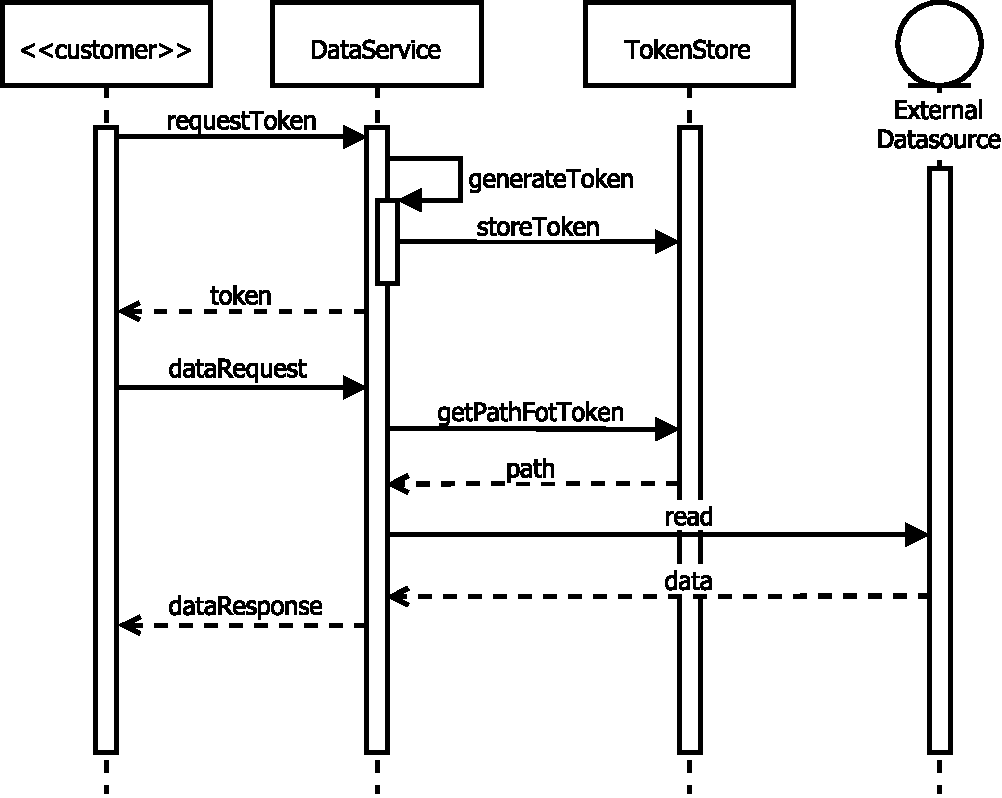
\includegraphics[width=0.8\textwidth]{SeqAccessSession}
    \caption{Ablauf: Datenfreigabe}
    \label{fig:seqaccesssession}
    \end{figure}




% -----------------------------------



\section{Implementation Algorithmus}



\section{Kommunikation}

Die Kommunikation zwischen den verschiedenen Service und Komponenten ist ein kritischer Faktor für die generelle Performance des gesamten Systems. Einerseits werden sehr viele Dateien über das Ne\-tz\-we\-rk übermittelt, andererseits muss damit ge\-rech\-net werden, dass einzelne Dateien Dateigrössen von 200 Megabyte überschreiten.

Recherche

Für den Transport über das Netzwerk sind \gls{Websocket}[s] eine erste Möglichkeit. Im Umgang mit kleinen Dateien sind \gls{Websocket}[s] eine einfache und schlanke Lösung. Für grosse Dateien sind sie alleine aber nicht ausreichend, da man schnell den verfügbaren Arbeitsspeicher überschreitet und auch die maximale String-Länge begrenzt ist. Für den Umgang mit grossen Dateien ist somit die Verwendung von \gls{Stream}[s] und \gls{Buffer}[s] Pflicht. 

Ein oft gesehenes weiteres Problem ist die Verwendung von \texttt{JSON\-.parse} und oder \texttt{JSON.stringify}.
Die Bibliothek \textit{bfj}\footnote{\url{https://github.com/philbooth/bfj}} kündigt an mit grossen Dateien arbeiten zu können, verwendet im Hintergrund aber die oben genannten Funktionen, welche nicht performant im Umgang mit grossen Dateien sind und zusätzlich ebenfallls auf die maximale String-Länge beschränkt sind.

Die Verwendung von \gls{Stream}[s] auf Basis von \gls{Websocket}[s] führ\-te mit der Bi\-blio\-thek \textit{websocket-stream}\footnote{\url{https://github.com/maxogden/websocket-stream}} leider ebenfalls nicht zum Erfolg. Da die Verwendung der verschiedenen \gls{Stream}[s] Probleme mit sich führte, wessen Ursprung nicht gefunden werden konnte.

Zu diesem Zeitpunkt war festgelegt, dass für die Übermittlung definitiv Streams verwendet werden müssen. Also konnte die Recherche weiter eingeschränkt werden.

\textit{Delivery.js}\footnote{\url{https://github.com/liamks/Delivery.js}} war die nächste interessante Bibliothek. Der Status \glqq Experimental\grqq war nicht der Grund für den Entscheid gegen diese Bibliothek. Vielmehr ist sie für eine Verwendung direkt mit \texttt{FileStreams}, also direkt mit der \texttt{I/O} vorgesehen. Zwar werden im Prototypen auch \texttt{FileStream} verwendet, jedoch werden die \gls{Stream}[s] nicht direkt über das Netzwerk weitergeleitet, sondern die einzulesenden Daten müssen zusätzlich noch verändert werden. \textit{Delivery.js} basiert auf \texttt{node-streams} und \texttt{socket.io}.

Identifizierte Probleme
\begin{enumerate}
    \item \textbf{Umgang mit grossen Dateien:} Grosse Dateien können aufgrund Begrenzungen des Arbeitsspeichers und oder Begrenzung der Datentypen nicht ohne weitere Schritte verwendet werden. Eine Lösung dafür ist die Verwendung von \gls{Stream}[s] und \gls{Buffer}[s].
    \item \textbf{Parsen und Serialisieren:} Die Übersetzung von rohe Binärdaten in ein Objekt und umgekehrt, ist bei grossen Dateien ebenfalls nicht trivial. \texttt{JSON.parse} und {JSON:stringify} funktionieren nicht ohne weiteres.
\end{enumerate}

\texttt{sockt.io}\footnote{\url{https://github.com/socketio/socket.io/}} ist eine viel versprechende Bibliothek. Sie ist in praktisch allen gängigen Programmiersprachen implementiert, darum gibt es auch zahlreiche Erweiterungen. Ebenfalls gibt es eine Erweiterung für die Verwendung von \gls{Stream}[s] namens \texttt{socket.io-stream}\footnote{\url{https://github.com/nkzawa/socket.io-stream}}.

Für die Serialisierung und das Parsen wird zusätzlich \texttt{msgpack}\footnote{\url{http://msgpack.org}} verwendet. Es arbeitet problemlos mit grossen Dateien.

Die \autoref{fig:kommunikation} zeigt die schlussendlich verwendeten Technologien im Überblick. Die Grundlage der Kommunikation zwischen \gls{ikc-core}, \texttt{DataService} und \texttt{IndexService} bildet \texttt{TCP/IP}. Darüber läuft das abhörsichere \texttt{HTTPS}-Protokoll. Im \texttt{JavaScript} wird die Bibliothek \texttt{socket.io} mit der oben erwähnten \gls{Stream}-Erweiterung verwendet. \texttt{msgpack} übersetzt die binären Rohdaten in Objekte und umgekehrt.



    \begin{figure}[H]
    \centering
    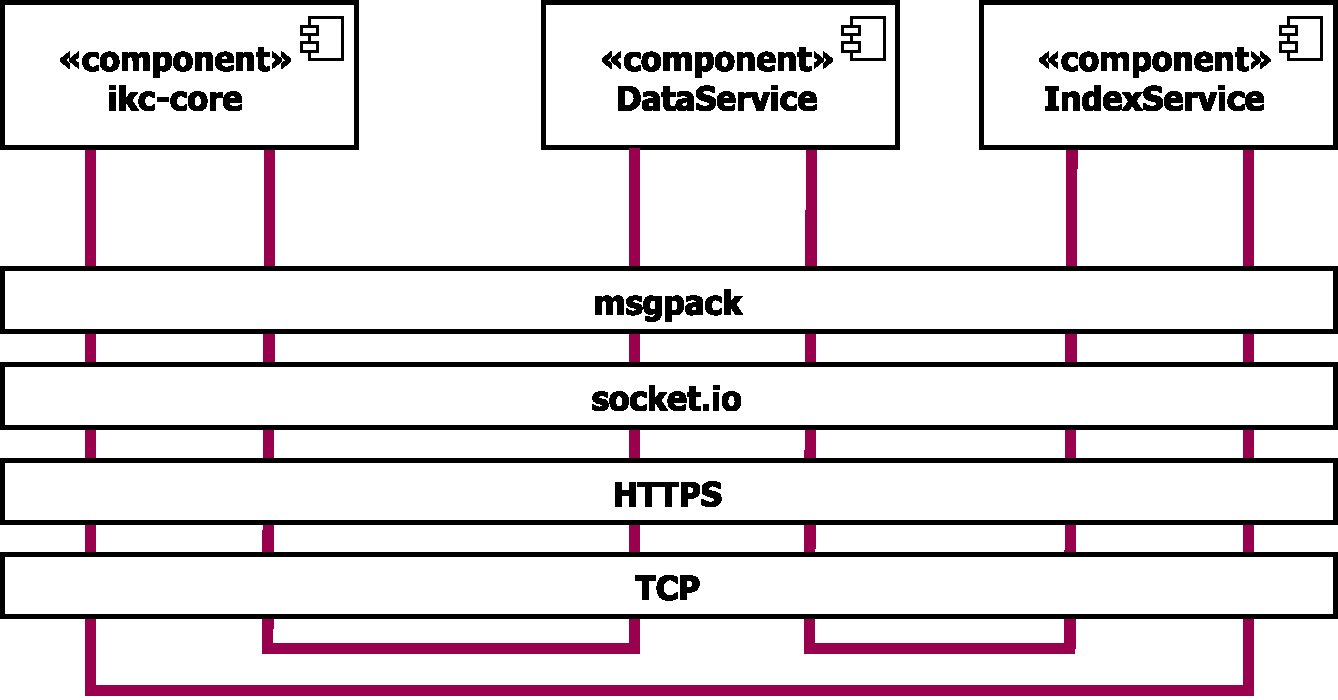
\includegraphics[width=1\textwidth]{ComponentDiagramm}
    \caption{Kommunikation}
    \label{fig:kommunikation}
    \end{figure}
    


\section{Protokoll}\label{section:protokoll}

Das Protokoll gibt an, in welchem Format die Daten übermittelt werden, sodass sie von beiden Seiten korrekt interpretiert werden. Es setzt also noch eine zusätzliche Ebene auf das obige Diagramm (\autoref{fig:kommunikation}) auf.


%    \begin{figure}[ht]
%    \centering
%    
\includegraphics[width=0.5\textwidth]{Protocol}
%    \caption{Protokoll Aufbau}
%    \label{fig:protocol}
%    \end{figure}

Die Kommunikation mit dem \texttt{IndexService} und dem \texttt{DataService} verläuft komplett eigenständig. Darum verwenden beide Services ein eigenes Protokoll. Für die Kommunikation mit einem Service muss das jeweilige Protkoll auch von der Gegenseite eingesetzt werden. Die Bedingung ist, dass alle übermittelnden Daten eine Instanz einer Klasse aus dem jeweiligen Protokoll sind.
    
%Diagramm Ablauf ala \url{http://www.hsg-kl.de/faecher/inf/netze/fehler2/index.php} 
%Diagramm Stack oder level evt. mit Diagramm  kabel mit verschiedenen schichten oder standard protocol stack \url{https://www.google.ch/url?sa=i&rct=j&q=&esrc=s&source=images&cd=&ved=0ahUKEwjJ5uO57drTAhUGvRoKHZIbBE4QjhwIBQ&url=http%3A%2F%2Fgeti2p.net%2Fnl%2Fdocs%2Fprotocol&psig=AFQjCNEHKXFjqJgGFF7pzQhblQm2WwWp6w&ust=1494145920025872}

Grundsätzlich besteht jede Nachricht aus einem Objekt der abstrakten Klasse \texttt{Mes\-sa\-ge}. Es stammt vorzugsweise aus der \texttt{MessageFactory}, um die Erzeugung des Objektes zusätzlich zu entkoppeln. Eine \texttt{Mes\-sa\-ge} besteht immer aus 

\begin{itemize}
    \item \textbf{einer \texttt{UUID}},\\
    Diese identifiziert eine Nachricht eindeutig. Sie besteht aus einem zufällig generierten alphanumerischen Muster.
    \item \textbf{einem \texttt{MessageType}}\\
    Damit die Nachricht jederzeit und an allen dafür vorgesehen Orten richtig interpretiert werden kann, besitzt sie einen für den jeweiligen Zweck vorgesehenen Typ. Dieser gibt explizit an, wie die Nachricht aufgebaut ist und welchen Zweck sie hat.
    \item \textbf{und einem \texttt{Messagebody}}
    Dieser stellt der eigentliche Inhalt der Nachricht dar. Er enthält den für den jeweiligen Typ vorgesehenen Body.
\end{itemize}

Das Klassendiagram (\autoref{fig:messageClassDiagram}) zeigt den Aufbau der abstrakten Klasse \texttt{Message} noch etwas detaillierter auf. Wie man erkennen kann, handelt es sich beim \texttt{MessageBody} um ein \texttt{Interface}, beim \texttt{MessageType} um einen \texttt{Enumerator}. Der \texttt{MessageBody} kann somit jeweils eine für den Zweck passende Instanz halten. Eine abstrakte Klasse wird aus dem Grund eingesetzt, dass die \texttt{id} zwingend bei jeder Unterklasse gesetzt wird.

    \begin{figure}[H]
    \centering
    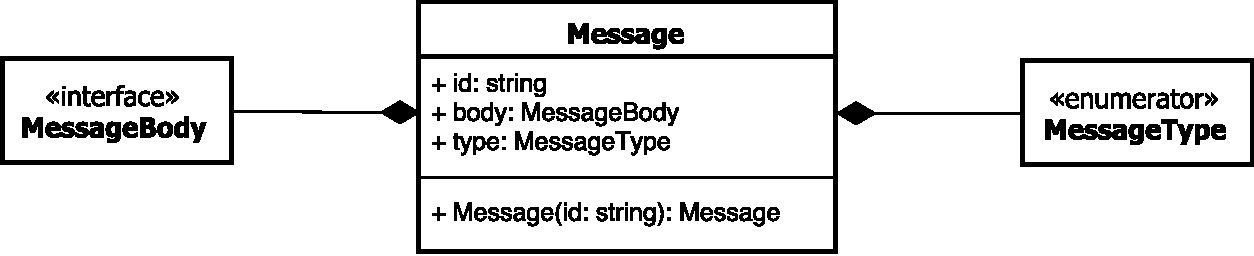
\includegraphics[width=1\textwidth]{MessageClassDiagram}
    \caption{Message Klassendiagram}
    \label{fig:messageClassDiagram}
    \end{figure}

\subsection{DataService-Protokoll}

\autoref{fig:dataclass} zeigt den Aufbau des \texttt{DataService}-Protokolls, dieses liegt im eigenen Paket \texttt{DataModel}. Dieses Protokoll wird im Prototyp für die Kommunikation zwischen \gls{ikc-core} und \texttt{DataService} beziehungsweise \texttt{IndexService} und \texttt{DataService} verwendet.

Im obigen Abschnitt (\autoref{section:protokoll}) wurde der Grundaufbau einer Nachricht aufgezeigt. Das \texttt{DataService}-Protokoll wird prinzipiell für den Datentransport eingesetzt. Das Protokoll gibt die dafür zu verwendenden Typen (\texttt{MessageTyp}) und Bodies (\texttt{MessageBody}) an. Die folgende Tabelle gibt einen Überblick über die verschiedenen Optionen. Zusätzlich zeigt das Ablaufdiagramm (\autoref{fig:seqdataprotocol}) einen vorstellbaren Beispielablauf mit den beteiligten Komponenten \gls{ikc-core} und \texttt{DataService}. Grundsätzlich folgt auf einen \texttt{Request} stets die entsprechende \texttt{Response}. Davon ausgenommen ist der Fehlerfall, wobei eine \texttt{ErrorResponse} zurückgeliefert wird.

\begin{longtable}{|p{4cm}| p{8cm}|}
  \hline
    \textbf{Bezeichnung} & \textbf{Beschreibung}\\\hline
    \texttt{TokenRequest} & Hierbei geht es um die Anfrage für eine Freigabe einer Datei oder eines Verzeichnisses. Für diesen Zweck gibt es das \texttt{Interface} \texttt{AccessSession} es enthält alle nötigen Zugangsdaten zur Verbindung mit einer externen Datenquelle. \newline
    
    Im Diagramm (\autoref{fig:seqdataprotocol}) ist die Klasse \texttt{SFTPAccessSession} enthalten. Diese regelt als Beispiel den Zugriff auf einen SFTP-Server.
    \\\hline
    \texttt{TokenResponse} &    
    Hat der \texttt{DataService} die Anfrage erhalten, schickt dieser bei Erfolg einen Token zurück. Dies geschieht in Form der \texttt{TokenResponse}. Diese enthält einen \gls{Token}. Dieser ist eine einmalige Zugriffsfreigabe für eine Datei oder einen Ordner von der jeweiligen Datenquelle.\newline
    
    
    Der \gls{Token} ist ein zufälliger generierter String, welcher auf dem \texttt{DataService} mit der jeweiligen \texttt{AccessSession} abgelegt ist.\\\hline
    \texttt{DataRequest} & Auf eine \texttt{TokenResponse} folgt ein \texttt{DataRequest}. Ist ein \gls{Token} auf dem \texttt{DataService} hinterlegt. Kann mit Hilfe dieses innerhalb eines \texttt{DataRequests} die jeweilige Datei oder das jeweilige Verzeichnis angefragt werden. \\\hline
    \texttt{DataResponse} & Die Antwort auf einen \texttt{DataRequest} ist im besten Fall eine \texttt{DataResponse}. Diese enthält den angefragten Dateiinhalt. \\\hline
    \texttt{ErrorResponse} & Schlägt bei einer der obigen Anfragen etwas fehl, wird eine \texttt{ErrorResponse} mit dem jeweiligen Fehler zurückgegeben. Fehlerursachen können von sehr unterschiedlicher Natur sein, beispielsweise sind Netzwerkprobleme oder falsche Zugangsdaten vorstellbar.\\\hline
        \caption{DataService: Message-Klassen}
    \label{dataservice-bodies}
\end{longtable}


    \begin{figure}[H]
    \centering
    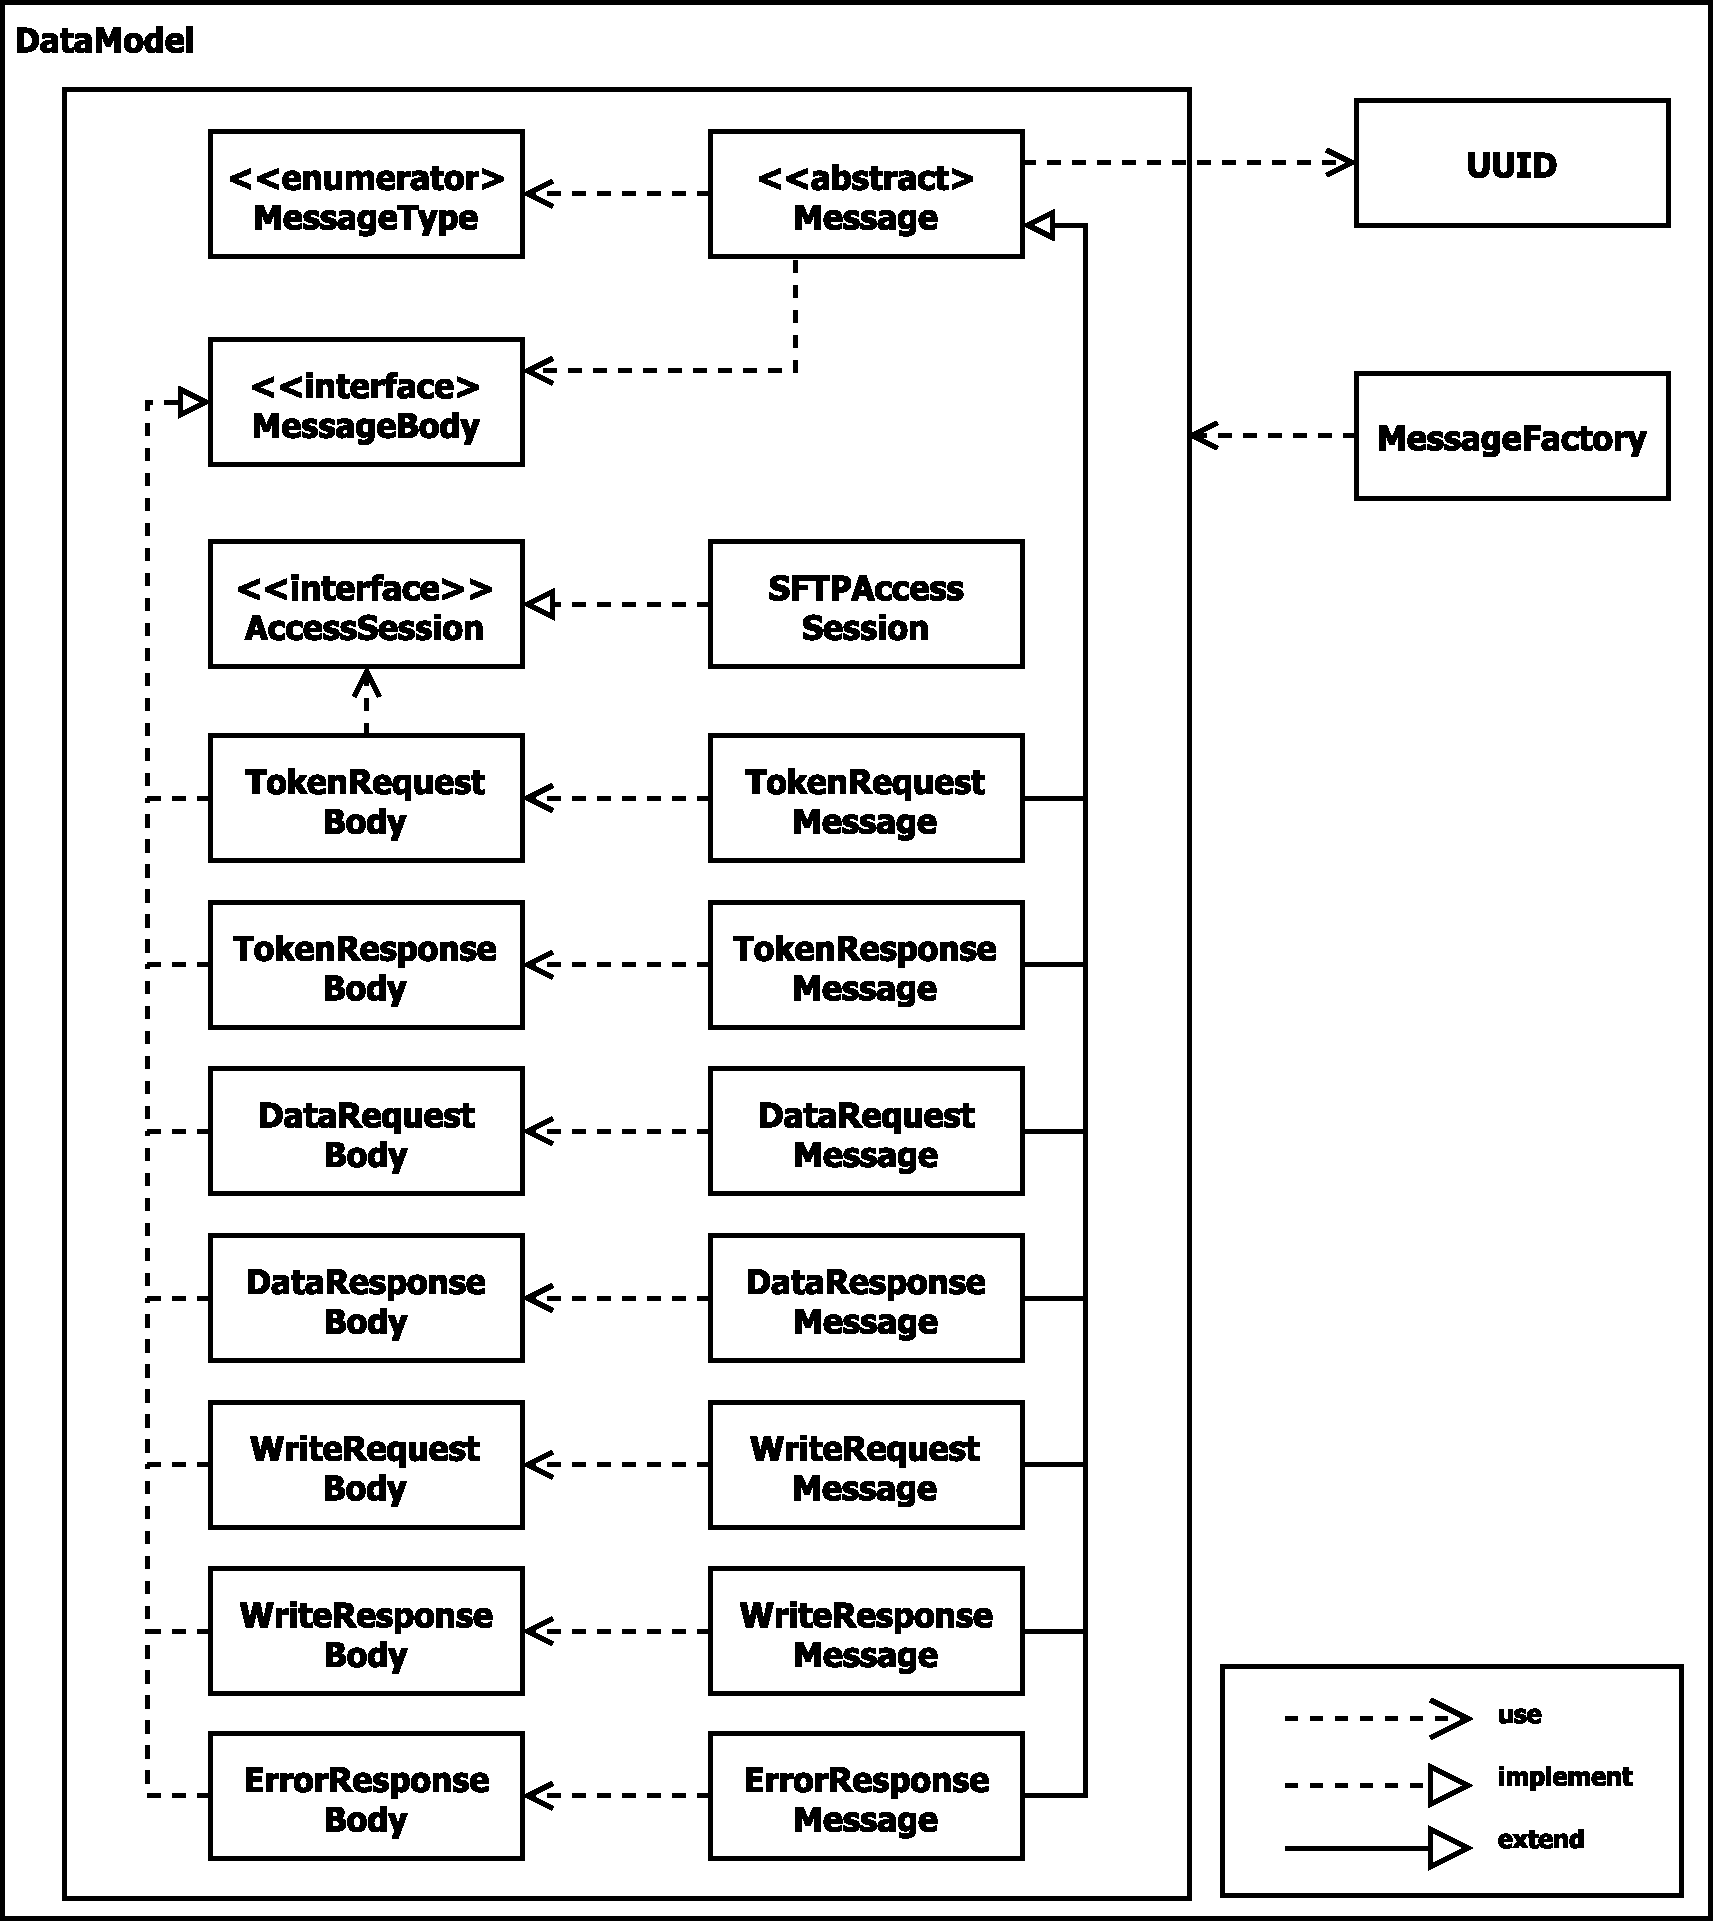
\includegraphics[width=0.9\textwidth]{DataModelClassDiagramm}
    \caption{Klassendiagramm DataService-Protokoll}
    \label{fig:dataclass}
    \end{figure}

    \begin{figure}[H]
    \centering
    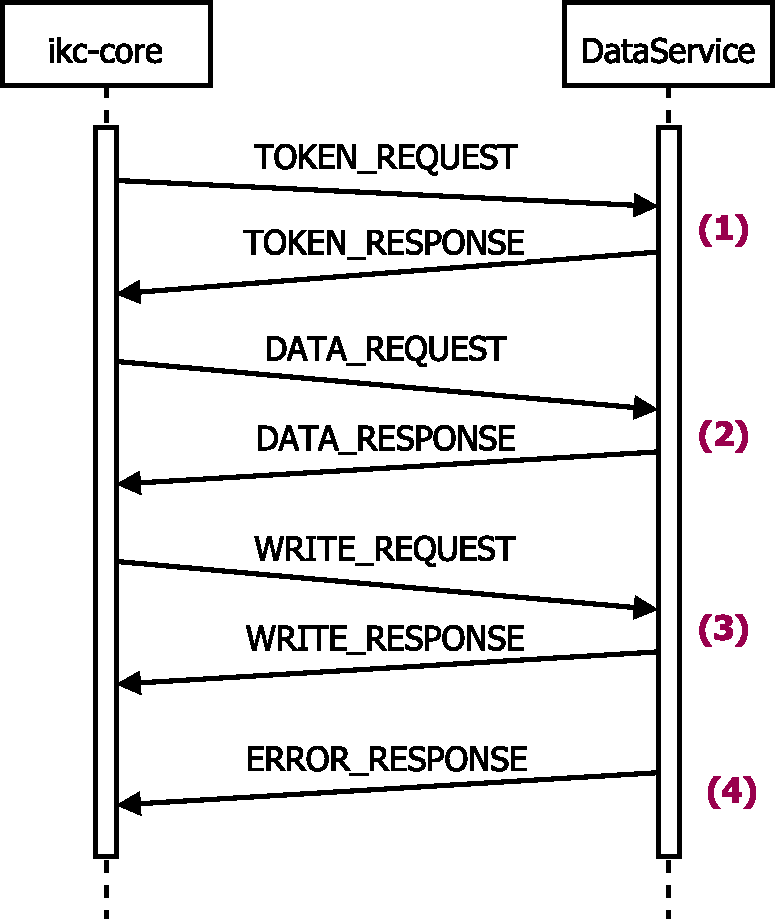
\includegraphics[width=0.5\textwidth]{DataModelSequence}
    \caption{Ablauf DataService-Protokoll}
    \label{fig:seqdataprotocol}
    \end{figure}


\subsection{IndexService-Protokoll}

Vom Aufbau her ähnlich wie das \texttt{DataService}-Protokoll sieht auch das \texttt{IndexService}-Protokoll aus (\autoref{fig:indexclass}). Wiederum ist die abstrakte Klasse \texttt{Message} die Grundlage. Allerdings unterscheiden sich die \texttt{Mes\-sa\-ge\-Typ\-es} und \texttt{MessageBodies}. Die Nachrichten haben hier den Zweck alle für die Volltextsuche und die Schlüs\-sel\-wort-\-Ex\-trak\-tion erforderlichen Daten zur Verfügung zu stellen.

    
    \begin{figure}[H]
    \centering
    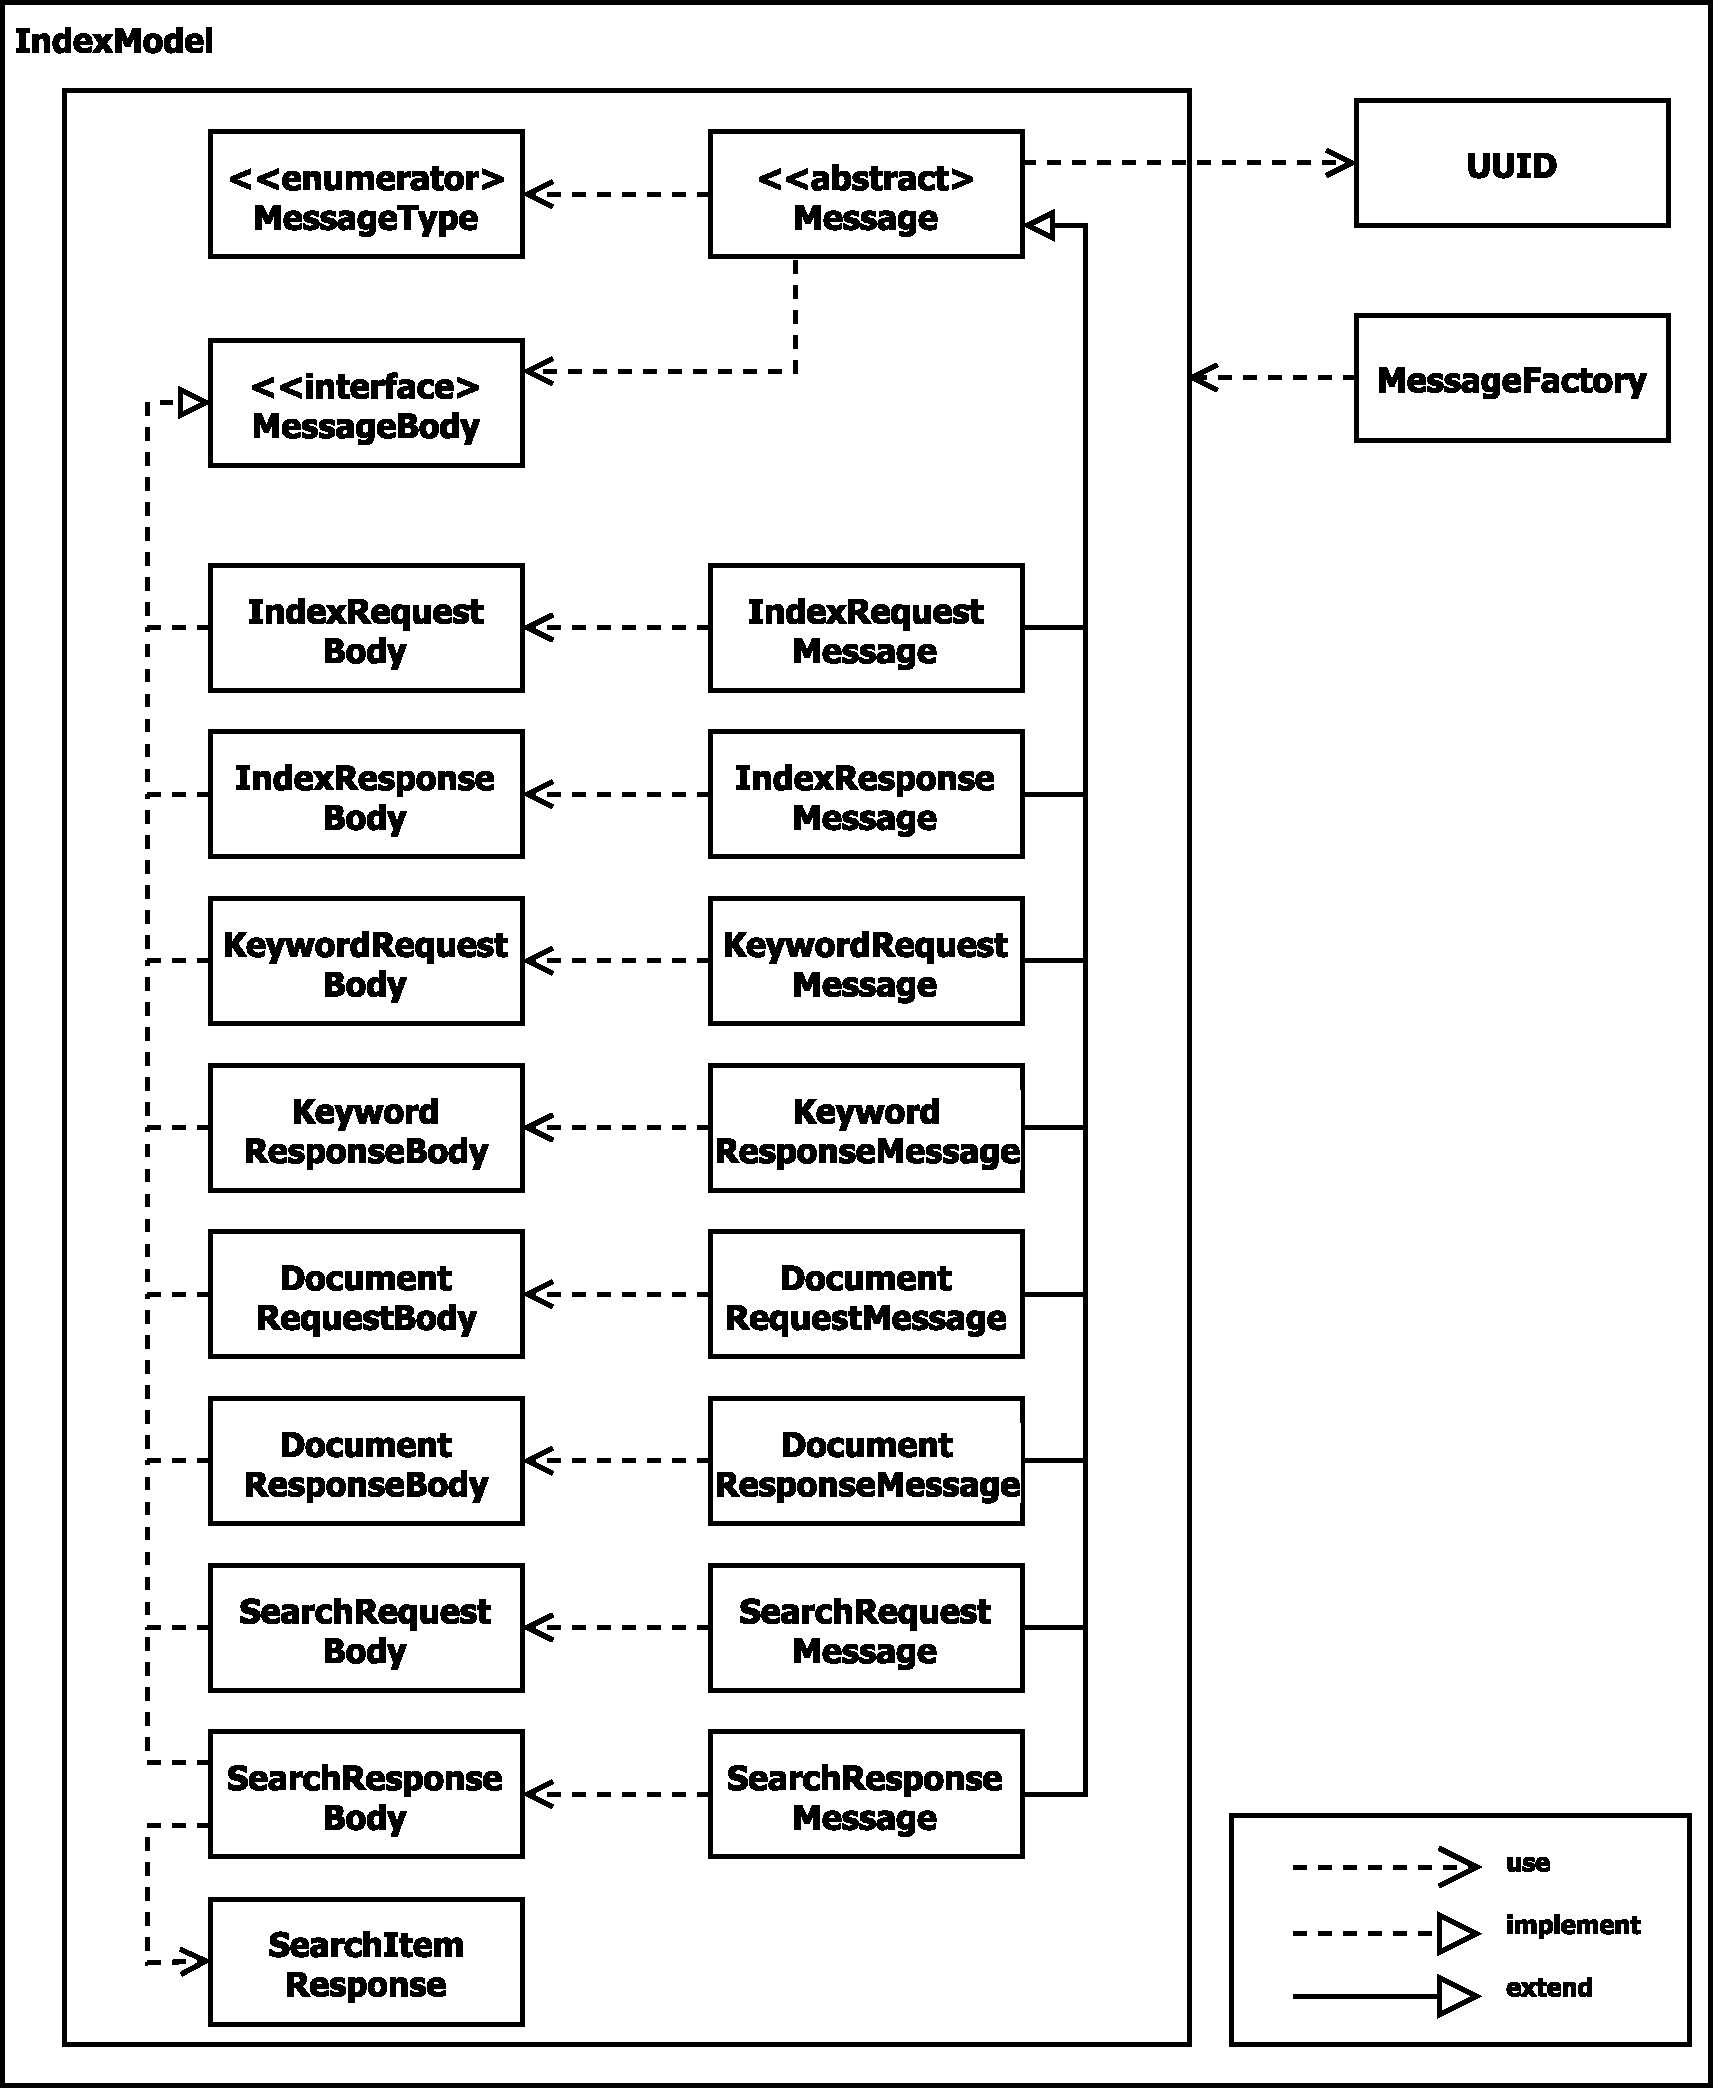
\includegraphics[width=1\textwidth]{IndexModelClassDiagramm}
    \caption{Klassendiagramm IndexService-Protokoll}
    \label{fig:indexclass}
    \end{figure}

Die Grundlage für die weiteren Vorgänge ist der Volltextindex. Dieser kann gelesen und persistiert werden. Ist diese Voraussetzung gegeben, können Schlüsselwörter für ein Dokument angefragt, zu einem Schlüsselwort passende Dokumente angefragt und Sucheresultate für einen bestimmten Begriff angefragt werden. Die Abläufe sind in der \autoref{fig:seqindexprotocol} ersichtlich. Die Vorgänge werden in folgender Tabelle genauer erläutert.

\begin{longtable}{|p{4cm}| p{8cm}|}
  \hline
    \textbf{Bezeichnung} & \textbf{Beschreibung}\\\hline
    \texttt{IndexRequest} & Der \texttt{IndexRequest} dient zum Anfragen des Volltextindex. Für diesen Vorgang wird zunächst der \gls{Token}, welcher zuvor beim \texttt{DataService} angefragt wurde, mitgeliefert. Zusätzlich dazu liegt der \texttt{Host} des anzufragenden \texttt{DataService} und die \texttt{indexId} ist die Identifikationsnummer des Index, falls dieser schon zuvor angefragt wurde.\\\hline
    \texttt{IndexResponse} & Nach der vorgängigen Anfrage für einen Index, folgt die Antwort in Form einer \texttt{IndexResponse}. Einziger Inhalt ist die \texttt{indexId} in Form eines Strings, welche den Index eindeutig identifizierbar macht.\\\hline
    \texttt{KeywordRequest} & Für die Schlüsselwort-Extraktion werden die Schlüsselwörter eines jeden Dokuments benötigt. Dafür gibt es den Vorgang \texttt{KeywordRequest}. Für die Verarbeitung werden ein \texttt{token} und ein \texttt{indexId} mitgeliefert. Der \texttt{token} hat seinen Ursprung wiederum im \texttt{DataService}. Er dient dazu den Volltext der jeweiligen Datei anzufragen. Die \texttt{indexId} ist wiederum dafür dazu da den gewünschten Index zu identifizieren.\\\hline
    \texttt{KeywordResponse} & Nach der obigen Anfrage folgt die Antwort in Form einer \texttt{KeywordResponse}. Diese beinhaltet ein Array von Strings, welches die extrahierten Schlüsselwörter des Dokumentes beinhaltet und die Identifikationsnummer des jeweiligen Dokumentes.\\\hline
    \texttt{DocumentRequest} & Sollen zu einem Schlüsselwort passende Dokumente angefragt werden, wird der \texttt{DocumentRequest} benutzt. Diese Anfrage beinhaltet das gesuchte Schlüsselwort und die Identifikationsnummer des jeweiligen Index.\\\hline
    \texttt{DocumentResponse} & Die Antwort beinhaltet wiederum das zuvor gesuchte Schlüsselwort und die Resultate als Array von Resultaten. Ein Resultat enthält den Titel, den Pfad, die Identifikationsnummer und den Inhalt des Dokumentes im Volltext.\\\hline
    \texttt{SearchRequest} & Eine weitere Funktionalität ist die Volltextsuche. Auch für diesen Zweck gibt es wiederum eine eigene Klasse. Um eine Suchanfrage abzusetzen, wird der Suchbegriff, eine Suchanfrage-Identifikationsnummer und wiederum eine \texttt{indexId} benötigt.\\\hline
    \texttt{SearchResponse} & Als Antwort auf eine Suchanfrage folgt ein Array von Suchresultaten. Ein Suchresultat enthält die Identifikationsnummer, den Pfad, den Titel und den Inhalt des gefundenen Dokuments.\\\hline
        \caption{IndexService: Message-Klassen}
    \label{indexservice-bodies}
\end{longtable}

    \begin{figure}[H]
    \centering
    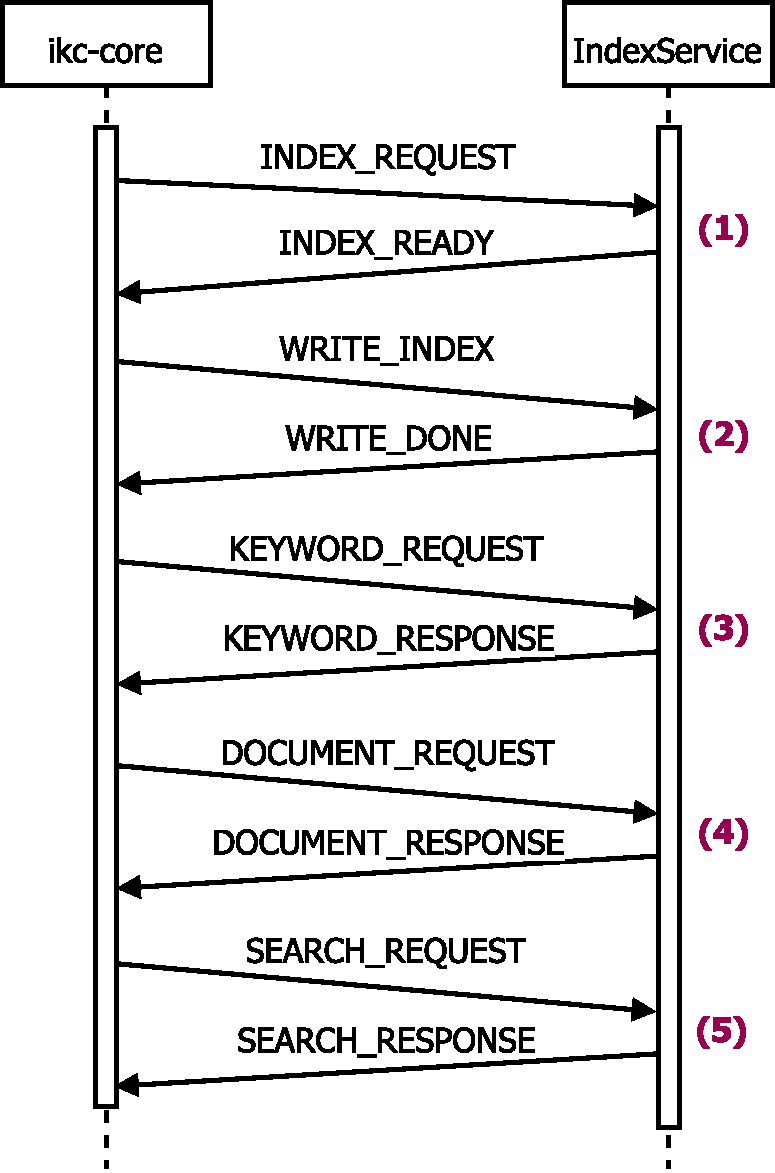
\includegraphics[width=0.5\textwidth]{IndexModelSequence}
    \caption{Ablauf IndexService-Protokoll}
    \label{fig:seqindexprotocol}
    \end{figure}
    
\section{Datenquelle}

Als Datenquelle wird eine vom Auftraggeber zur Verfügung gestellte Sammlung von etwas mehr als 100'000 Wikipedia Artikeln verwendet. Diese enthalten qualitativ hochwertige Informationen in Volltext und bilden die Grundlage für die Schlüsselwort-Extraktion und die Volltextsuche.

\section{Persistenz}

Im Gegensatz zum bestehenden Prototypen aus dem Forschungsprojekt \gls{IKC}, wird in dem hier vorliegenden als Datenquelle zusätzlich \gls{SFTP} ergänzt. Dies hat mitunter den Grund, wie in Absprache mit dem Auftraggeber festgelegt wurde, dass die erweiterte Anbindung an Cloud-Dienste, wie etwa Dropbox und Evernote, nicht der Kern dieser Bachelor-Arbeit ist. Der Fokus dieser Arbeit ist \textit{Information Retrieval} mittels \textit{Natural Language Processing} auf Basis von Schlüsselwort-Extraktion. Daher soll auch in diesem Bereich der Grossteil der zur Verfügung stehenden Zeit investiert werden. 

Aus diesem Grund werden die zu indexierenden Dateien, wie auch die Indizes und eventuelle Konfigurationsdateien auf einem \gls{SFTP}-Server gehalten.

\gls{SFTP} (SSH File Transfer Protocol) basiert auf \gls{SSH}, daher kann für die Authentifizierung direkt auch mit \gls{SSH}-Schlüssel gearbeitet werden. Für eine Verbindung mit einem \gls{SFTP}-Server sind folgende Daten notwendig:


\begin{longtable}{|p{4cm}| p{8cm}|}
  \hline
    \textbf{Bezeichnung} & \textbf{Beschreibung}\\\hline
    \texttt{host} & Dies entspricht dem Host-Namen oder der IP-Adresse der Servers, mit welchem verbunden werden soll.\\\hline
    \texttt{port} & Der Port gibt an, auf welchem Port der \gls{SFTP}-Server auf die Verbindung wartet. \gls{SSH} läuft standardmässig auf Port 22, dieser wird auch hier als Standardwert angenommen.\\\hline
    \texttt{user} & Dies ist der Benutzernamen für den Zugang zum Server. Dieser hat üblicherweise sein Verzeichnis auf dem jeweiligen Server.\\\hline
    \texttt{keyPath} & Wie oben schon erwähnt, wird für die Anmeldung kein Passwort, sondern direkt ein SSH-Private-Key verwendet. Der Dateipfad dazu wird hier angegeben.\\\hline
    \texttt{docDir} & Will der Benutzer nicht direkt mit seinem Stammverzeichnis arbeiten, hat er hier die Möglichkeit ein anderes Verzeichnis anzugeben. Die entsprechenden Berechtigungen dafür sind vorausgesetzt.\\\hline
        \caption{SFTP: Anmeldedaten}
    \label{sftp-anmeldung}
\end{longtable}


In \autoref{ssh-connection} sind die oben besprochenen Angaben zusätzlich in \gls{Typescript} ersichtlich. Das Objekt \texttt{config} enthält alle für die Verbindung nötigen Daten. Diese wurden in der Entwicklung des Prototypen so verwendet. Der Wert \texttt{docDir} zeigt hier auf das Verzeichnis des Benutzers \texttt{ikcdata}. Diese musste hier zusätzlich gesetzt werden, da der Benutzer Zugriff auf das Stammverzeichnis des Server hat. Ohne eine zusätzliche Angabe würde der Service direkt auf dieses Verzeichnis zugreifen.


\begin{listing}[H]
\inputminted[
frame=lines,
framesep=2mm,
baselinestretch=1.2,
linenos,
breaklines=true
]{js}{sourcecode/dataservice/ssh-connection.ts}
\caption{SSH-Verbindung}
\label{ssh-connection}
\end{listing}

Auf Zeile 1 (\autoref{ssh-connection}) ist die für die Verbindung verwendete Bibliothek \texttt{ssh2}\footnote{\url{https://github.com/mscdex/ssh2}} zu sehen.


\begin{listing}[H]
\inputminted[
frame=lines,
framesep=2mm,
baselinestretch=1.2,
linenos,
breaklines=true,
firstline=6, 
lastline=33,
highlightlines={7, 21-24}
]{js}{sourcecode/dataservice/ssh-sftp.ts}
\caption{SSH: SFTP-Client}
\label{ssh-sftp}
\end{listing}


Die Bibliothek liefert nach dem Aufbau der \gls{SSH}-Verbindung zum Server ein \gls{SFTP}\gls{Stream}-Objekt zurück (\autoref{ssh-sftp} Zeilen 21-24)\footnote{Dokumentation zu Client-Methoden \url{https://github.com/mscdex/ssh2}}. Dieser \gls{Stream} bietet die gewünschte Funktionalität zum Lesen und Schreiben von Verzeichnissen oder Dateien.\footnote{\url{https://github.com/mscdex/ssh2-streams/blob/master/SFTPStream.md}} Selbstverständlich kann die zugrundeliegende \gls{SSH} auch direkt weiterverwendet werden. Dies ermöglichst beispielsweise eine einfache Auswertung und schnellen Vergleich über externe Änderungen auf Datei-Ebene.


\subsection{Auto-Indexierung}

Da SSH Zugriff, ls -a und TimeStamp mit Map vergleichen..

    
\section{Index-Berechnung}

Die Berechnung des Index ist eine der prozessorintensiven Aufgaben, sie ist Zeit- und Ressourcen-intensiv. Dies insbesondere aufgrund der vielen Lese-Zugriffe. Darum wird der Index wann immer möglich zwischengespeichert, sodass eine erneute Berechnung erspart bleibt. Sie bildet die Grundlage für die zentralen Funktionen (\gls{Keyword}-Ex\-trak\-tion und Suche) des Prototypen.  

\autoref{fig:seqindexalreadybuilt} zeigt den aufwändigeren Ablauf. 
\begin{itemize}
    \item \texttt{requestIndex}: Der \gls{ikc-core} möchte Zugriff auf den Index. Dafür tätigt er eine Anfrage beim \texttt{IndexService}. Der \texttt{IndexService} hat den Index nicht geladen, er startet also die Berechnung.
    \item \texttt{dataRequest}: Dafür müssen zunächst alle Dokumente eingelesen werden. Dafür muss eine Anfrage an den \texttt{DataService} gemacht werden.
    \item \texttt{dataResponse}: Diese wird mit den geforderten Daten beantwortet.
    \item \texttt{parseData}: Die Daten werden geparst damit sie weiterverarbeitet werden können.
    \item \texttt{addDocToIndex}: Nun wird jedes einzelne Dokument, dem Index hinzugefügt.
    \item \texttt{indexReady}: Dem \gls{ikc-core} wird gemeldet, dass der Index bereit ist.
\end{itemize}

    \begin{figure}[H]
    \centering
    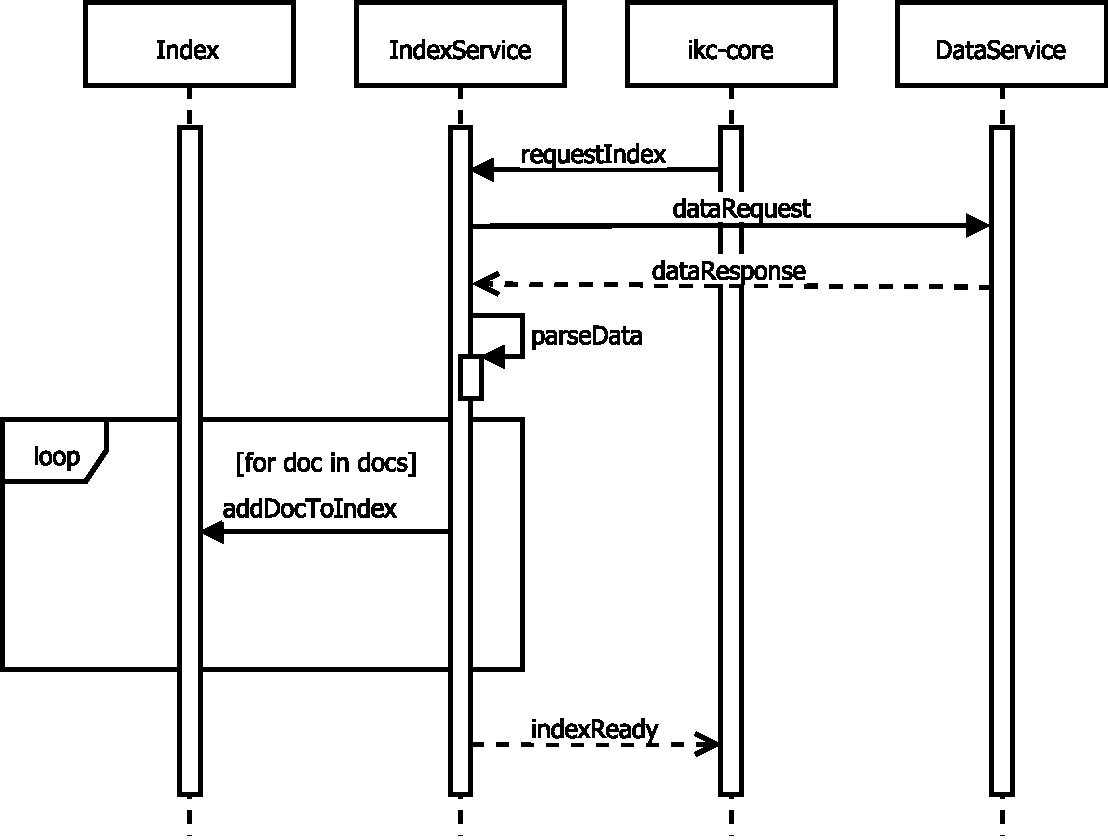
\includegraphics[width=0.7\textwidth]{SeqIndexLoad}
    \caption{Ablauf: Index-Berechnung}
    \label{fig:seqindexload}
    \end{figure}

Falls ein Index bereits berechnet und persistiert wurde, muss er nur noch eingelesen werden. Diesen Ablauf wird in der \autoref{fig:seqindexalreadybuilt} erläutert. 
\begin{itemize}
    \item \texttt{requestIndex}: Der \gls{ikc-core} möchte Zugriff auf den Index. Dafür tätigt er eine Anfrage beim \texttt{IndexService}. Der \texttt{IndexService} hat den Index nicht geladen, er startet also die Berechnung.
    \item \texttt{dataRequest}: Nun muss das serialisierte Index-Objekt geladen werden. Dafür muss eine Anfrage an den \texttt{DataService} gemacht werden.
    \item \texttt{dataResponse}: Diese wird mit den geforderten Daten beantwortet.
    \item \texttt{parseData}: Die Daten werden geparst und verarbeitet.
    \item \texttt{loadIndex}: Der Index wird in den Arbeitsspeicher geladen.
    \item \texttt{indexReady}: Dem \gls{ikc-core} wird gemeldet, dass der Index bereit ist.
\end{itemize}

    \begin{figure}[H]
    \centering
    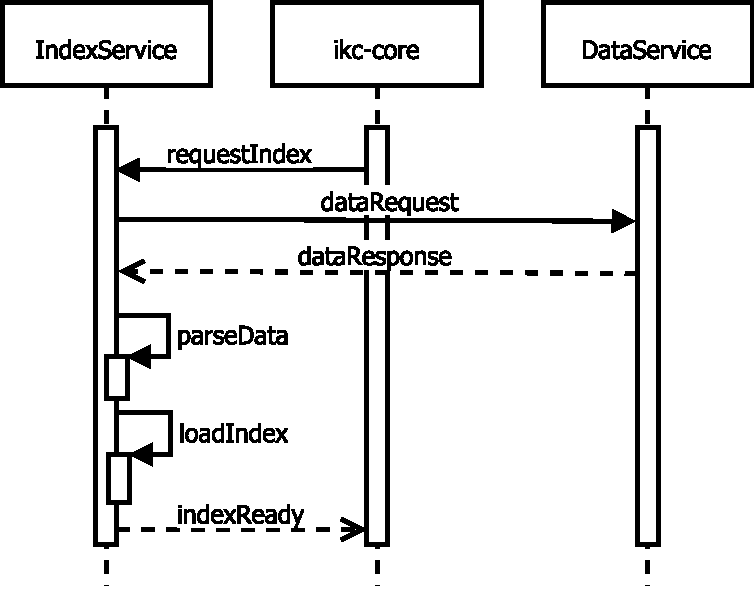
\includegraphics[width=0.8\textwidth]{SeqIndexLoadAlreadyBuilt}
    \caption{Ablauf: Index-Berechnung}
    \label{fig:seqindexalreadybuilt}
    \end{figure}
    
    
Die \autoref{fig:seqindexloadalreadydone} hingegen zeigt den Ablauf, falls der Index schon im \texttt{IndexService} geladen ist.

\begin{itemize}
    \item \texttt{requestIndex}: Der \gls{ikc-core} benötigt den Index. Dafür fragt er den \texttt{IndexService} an. Dieser hält den Index schon im Arbeitsspeicher bereit.
    \item \texttt{indexReady}: Somit kann er diesen direkt zurückliefern.
\end{itemize}
    
    \begin{figure}[H]
    \centering
    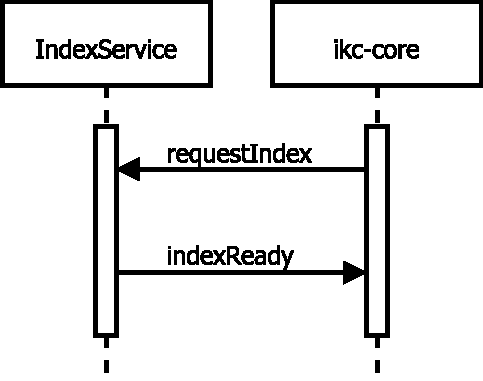
\includegraphics[width=0.5\textwidth]{SeqIndexLoadAlreadyDone}
    \caption{Ablauf: Index-Zugriff}
    \label{fig:seqindexloadalreadydone}
    \end{figure}

\section{Keyword-Extraktion}
Die \gls{Keyword}-Extraktion ist eine der wichtigsten Funktion des Prototypen. In der nachfolgenden \autoref{fig:seqkeywordextraction} wird der Ablauf genauer erläutert:
\begin{itemize}
    \item Initiert wird die Extraktion von \gls{Keyword}[s] durch die \texttt{KeywordRequest} Nachricht, welche der \gls{ikc-core} an den \texttt{IndexService} sendet. Anschliessend wir das entsprechende Dokument von dem \texttt{DataService} bezogen und für die verarbeitung Aufbereitet. 
    \item Innerhalb des \texttt{IndexService} werden die relevanten \gls{Keyword}[s] innerhalb des \texttt{InformationExtractor} berechnet und zurückgegeben. 
    \item Anschliessend werden diese innerhalb einer \texttt{KeywordResponse} Nachricht an den \gls{ikc-core} gesendet.
\end{itemize}

    \begin{figure}[H]
    \centering
    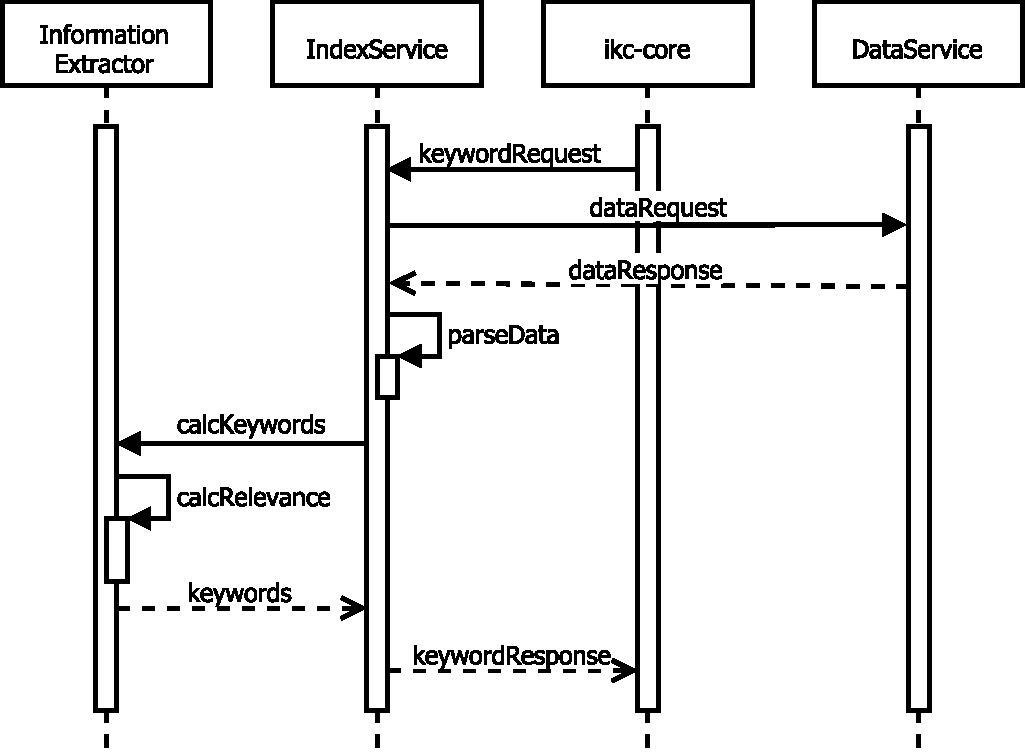
\includegraphics[width=1\textwidth]{SeqKeyword}
    \caption{Ablauf: \gls{Keyword} Extraktion}
    \label{fig:seqkeywordextraction}
    \end{figure}

\section{Dokument-Extraktion}
Neben der Extraktion von \gls{Keyword}[s] sollen pro \gls{Keyword} auch passende Dokumente extrahiert werden. Dieser Ablauf ist in der \autoref{fig:seqdocument} ersichtlich.
\begin{itemize}
    \item der \gls{ikc-core} fordert durch eine \texttt{DocumentRequest} eine Liste von Dokumente für ein \gls{Keyword} an. 
    \item Anschliessend extrahiert der \texttt{InformationExtractor} eine Liste von passenden Dokumente und bewertet ihre Relevanz. 
    \item Innerhalb einer \texttt{DocumentResponse} Nachricht wird die resultierende Liste an den \gls{ikc-core} gesendet und die Anfrage somit beendet.
\end{itemize}

    \begin{figure}[H]
    \centering
    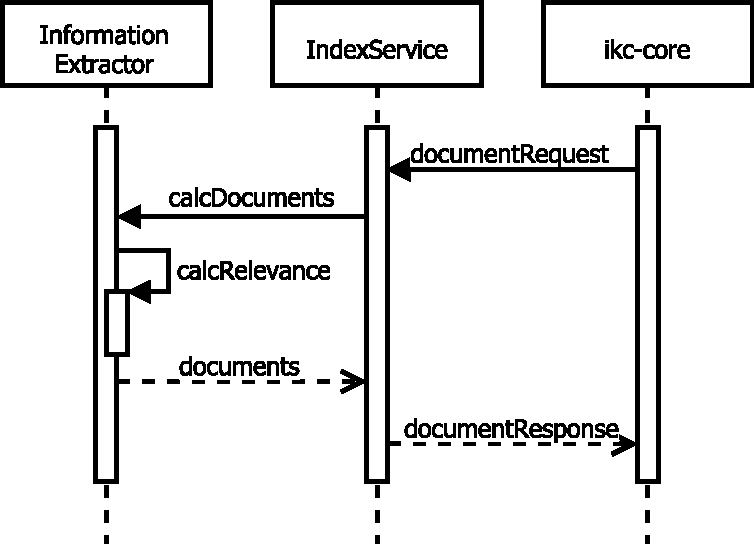
\includegraphics[width=1\textwidth]{SeqDocument}
    \caption{Ablauf: Dokument Extraktion}
    \label{fig:seqdocument}
    \end{figure}

\section{Suche}
Um ganze Datenquellen zu durchsuchen wird eine Volltext Suche verwendet. Mit Hilfe der folgenden \autoref{fig:seqsearch}, wird der Ablauf der Suche aufgezeigt:
\begin{itemize}
    \item Innerhalb des \gls{ikc-core} wird eine Suchanfrage abgesetzt. Diese erreicht den \texttt{IndexService} eingebetet in einer \texttt{SearchRequest} Nachricht. 
    \item Intern arbeitet die \texttt{Search} die Suche ab und liefert die entsprechenden Resultate.
    \item Die Resultate werden anschlissend in einer \texttt{SearchResponse} Nachricht eingebettet an den \gls{ikc-core} gesendet.
\end{itemize}

    \begin{figure}[H]
    \centering
    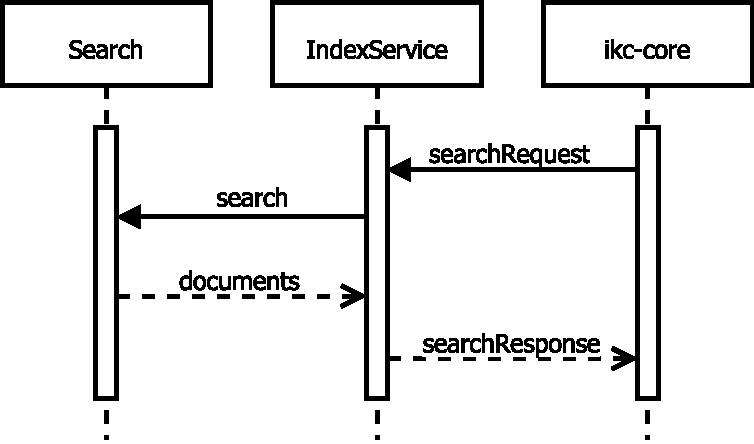
\includegraphics[width=0.7\textwidth]{SeqSearch}
    \caption{Ablauf: Suche}
    \label{fig:seqsearch}
    \end{figure}




\section{Benutzerhandbuch}